\documentclass[11pt,fleqn,twoside]{article}
\usepackage{makeidx}
\makeindex
\usepackage{palatino} %or {times} etc
\usepackage{plain} %bibliography style
\usepackage{amsmath} %math fonts - just in case
\usepackage{amsfonts} %math fonts
\usepackage{amssymb} %math fonts
\usepackage{lastpage} %for footer page numbers
\usepackage{fancyhdr} %header and footer package
\usepackage{mmpv2}
\usepackage{url}
\usepackage{graphicx}
\usepackage{moreverb}
\usepackage{framed}
% the following packages are used for citations - You only need to include one.
%
% Use the cite package if you are using the numeric style (e.g. IEEEannot).
% Use the natbib package if you are using the author-date style (e.g. authordate2annot).
% Only use one of these and comment out the other one.
\usepackage{cite}
%\usepackage{natbib}

\begin{document}

\name{Daniel Atkinson}
\userid{daa9}
\projecttitle{Arduino based obstacle avoidance robot}
\projecttitlememoir{Obstacle avoidance robot} %same as the project title or abridged version for page header
\reporttitle{Progress Report}
\version{1.0}
\docstatus{Final}
\modulecode{CS39440}
\supervisor{Dave Barnes} % e.g. Neil Taylor
\supervisorid{dpb}
\wordcount{3211}

%optional - comment out next line to use current date for the document
\documentdate{17 November 2012}
\mmp

\setcounter{tocdepth}{3} %set required number of level in table of contents
\tableofcontents

\newpage

%==============================================================================
\section{Project Summary}
%==============================================================================
\subsection{Aim}
The aim of the project is to build and program an autonomous robot that can move around freely within an environment and avoid coliding with obstacles it may find.
\subsection{Background}
I tend to experiment with electronic components on a regular basis.  Due to this I try and make small systems and get them working, originaly nothing more than a simple timer or an audio amplifier.  Naturaly the progression from this would be to move onto microcontrollers.
\\I like to see things move, it keeps my interest.  The satisfaction I get when having started with nothing and going through to get something built and moving is what makes me think up new ideas, how can this be modified?, how can this be made better?.  A robotic project the perfect thing for me to do.
\subsection{Possible Application}
Many projects if not all in the field of autonomous robotics could benefit from some kind of obstacle avoidance system on board.  Even if it is just a failsafe to stop the device damaging itself on it environment as this would hinder its operation and may result in being very costly.  The easier robots to apply this kind of system to is one that does not rely on having a special shape for its operation \cite{snake} such as a snake robot.  Generaly blocky wheeled or track driven robots work best from this kind of system due to the amount of sensors required and their size is usualy fairly large.
\\Robots designed to go into environments where humans cannot normaly go would also benefit from a system where it can detect objects in proximity to itself or even automaticaly avoid colision.  These robots may be designed to traverse the interior of a flaming building to aid putting out the source of a fire, to clean up nuclear waste from a nuclear power station or even navigate the surface of another planet.
%==============================================================================
\section{Current Progress}
%==============================================================================
\subsection{Related Works}
There are already lots of examples of work in this area.  Cameras can be used to find a path between objects using different image proccessing techniques.  These require a fairly high level of processing due to the amount of data in each image.  This can also sometimes lead to mistaking visible patterns in the environment as obstacles or empty space when there is none, such as a mirror or a patterned carpet.
\cite{roborealm}
\subsubsection{Wrist Device}
I put a small amount of time into building a portable device to interact with the main robot with main the purpose of reading live debug output.  This device was thought of because following aroudn the prototype with a laptop plugged into it became very anoying and quite awkward because if the robot made a tight turn it could get tangled up in the cable.
\\This resulted in using some components I had lay around to build a temporary solution.  I used an Arduino fio, this has a built in LiPo battery socket, charging circuit and has an xbee module socket.  An xbee is a wireless radio popular with elecronics hobbyists for project such as this.  It provides a simple serial interface over wireless, exactly what I needed, Also a 2x16 character LCD display.
\\It's not pretty but it works for a temporary/initial solution.
\begin{figure}[h]
\centering
        \includegraphics[width=3.0in] {figures/mobile-board.png}
        \caption{Small wireless monitor}
        \label{Small wireless monitor}
\end{figure}
\clearpage
I had the intention to have this mounted on my wrist so I would not have to constantly have to pick it up and put it down to use.  A glove was used to hold it to my wrist.
\begin{figure}[h]
\centering
        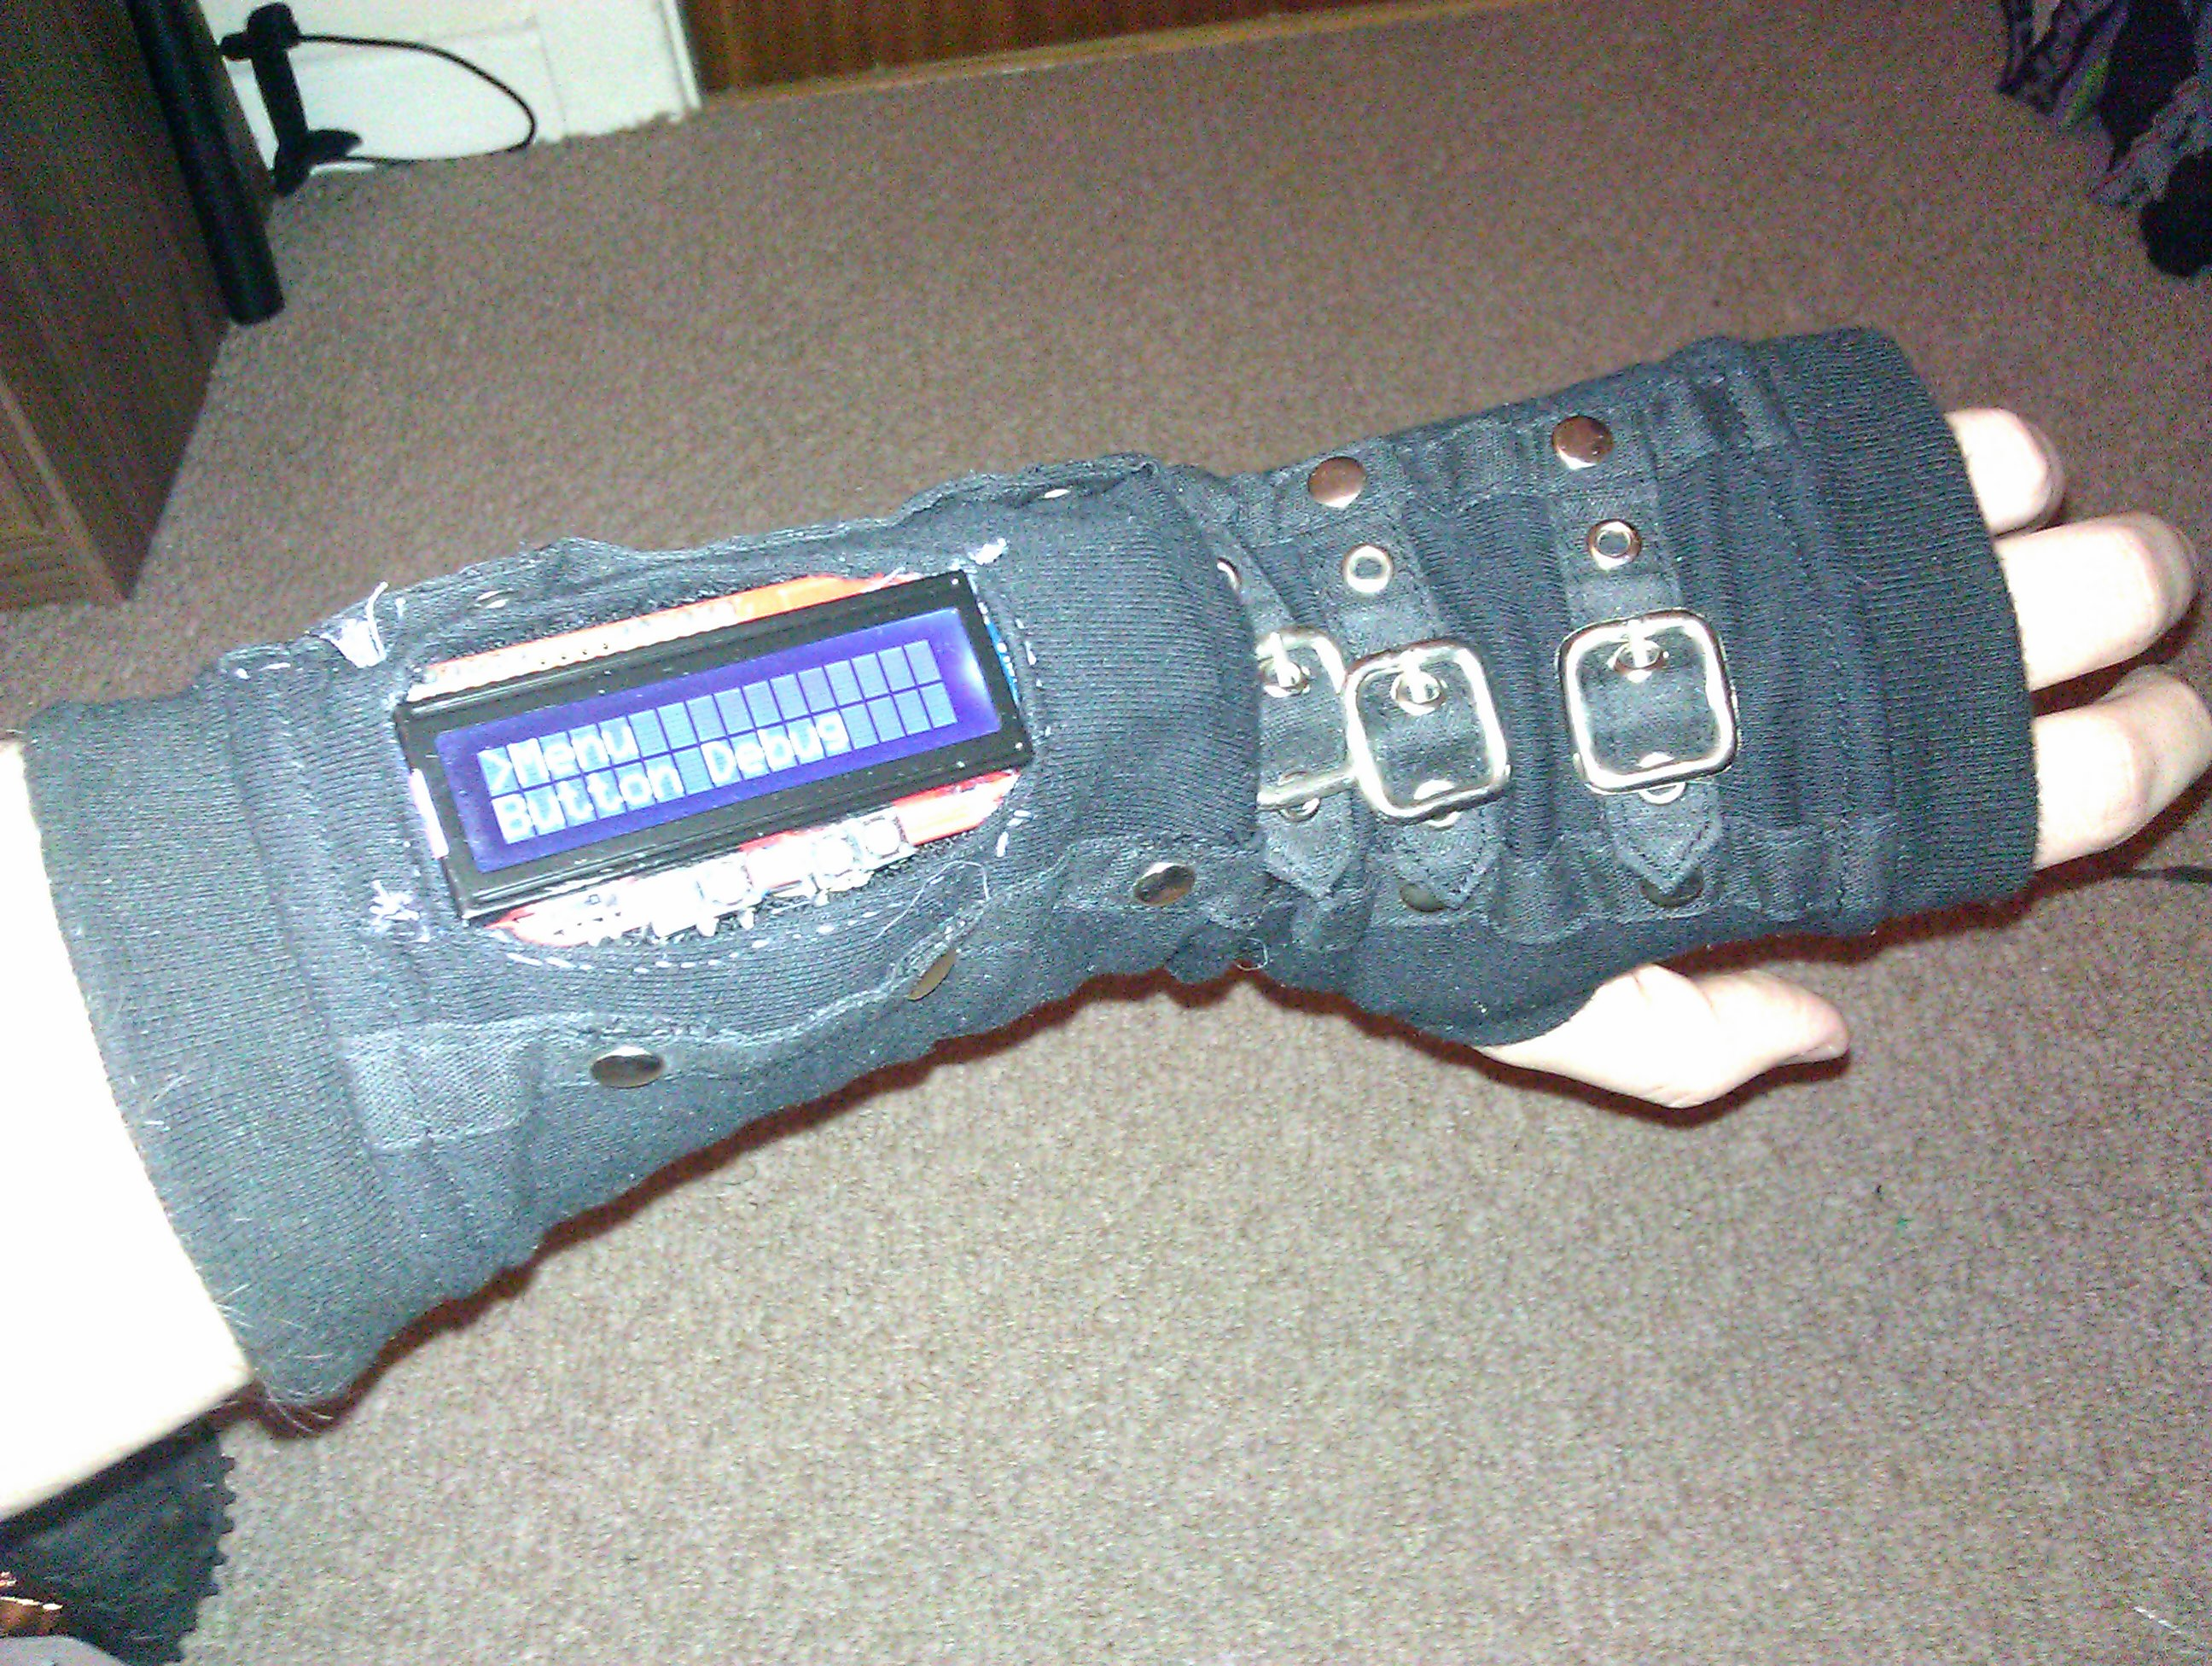
\includegraphics[width=4.0in] {figures/wrist-device.jpg}
        \caption{Wrist mounted device}
        \label{Wrist mounted device}
\end{figure}
\subsubsection{Pioneer}
I have had experience using the pioneer research robot created by Adept MobileRobots \cite{mobilerobots} these are the same robots as used in the robotics lab at Aberystwyth University.  The experience I had with these robots was using their ultrasonic sensors to try and avoid hitting some polystyrene boards.  Due to the limited time available to use the robots the resulting code was not very effective or polished but the experience heavily influenced the design of this project.  The two front drive wheels witht he rear caster to enable turning felt like a good fit for moving forwards to navigate through areas.  Adept Mobilerobots also make another model which is like a miniture version of the pioneer called the AmigoBot, this one is a closer match to my current design.
\subsection{Technologies}
Several different technologies will be taken advantage of for the duration of this project.  Some hardware and some software.
\subsubsection{Version Control}
This is majorly usefull in any project the involes storing code or documents digitaly.  It is even usefull just as a backup tool, to be save from accidental deletions, from hard drive failure, or any number of unfortunate occurances as you can just re-download or revert changes you have made.
\\A more useful way to use version control is to take advantage of its other features.  Features such as branching and merging.  These enable a person to make a branch of a project so that they can work on a specific feature independantly of the main project.  You may make multiple branches at the same time for working on different features and then when they are finished, merge them back into the main project.  Different version control systems ahve different algorithms that help with merging more inteliently, rather than asking you about every single line it is trying to put into a document.  Personaly I am using git as my version control system of choice.  This is mainly because I am more familiar with it than any of the other solutions and also because github\cite{github} %citation here%
give university student free private repositories.
\\Github also provides an easy to use web interface.  This interface also provides tools for displaying repository statistics, such as what times a user makes the majority of their commits or how much additions/deletions they do.
\begin{figure}[h]
\centering
        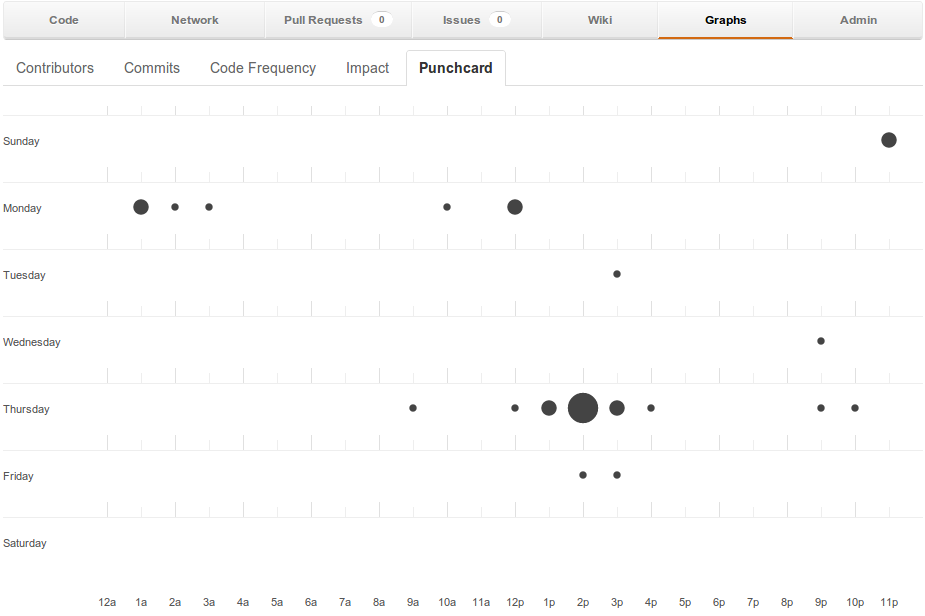
\includegraphics[width=4.0in] {figures/punchcard.png}
        \caption{Project punchcard}
        \label{Project punchcard}
\end{figure}
\\Github also provides hosting for a project website which is automaticaly built from a branch inside your repository.  I have purchased a domain and host a public summary of the project as the forward facing page of this private repositoy, it is located at "fyp.tria.me".  Fyp stands for final year project, tria is just the name I have given the robot.
\clearpage
\subsubsection{Sensors}
\begin{itemize}
\item LDR (light dependant resistor)
\\Small resistor that changes its resistance depending on how much light it is exposed to.
\\This could be used to detect if the robot is very close to bumping into an object and avoid it as the object would shadow some of the light from getting to the resistor, like a bump skirt.
\item Camera
\\A camera could be used to detect objects in front of it using various image processing techniques.  This method is good because it can potentialy map a relatively large area in a single image.  On the other hand it requires more processing to do which can be slow and result in having colided into an object or being stuck in a tight space before it has finished processing. A camera and the proccessing linked to using it for obstacle avoidance also increases power consumption, decreasing total runtime.
\item Infra Red
\\Used to detect distance from an object.  An emiter and a reciever linked to work like the light dependant resistor but using infra red instead of visible light.  Depending on intensity it can be used to detect distance.  These could be aranged all around the robot like a halo to detect objects from all sides.
\item Sonar
\\Again emiter, reciever style approach.  Emit an ultrasonic wave to bounce off of whatever is in  front of the emitter and then time how long it takes to be picked up by the reciever to determine how far away the object is.  This method comes with its drawbacks.  Due to how sound waves behave when they interact with the environment by bouncing off of it.  If the surface is angled or curved the sound can bounce away from the reciever, either not returning to it at all and giving a false reading of there beign nothing in front of it, or be bouncing off of multiple objects back to the reciever giving a false longer reading than there actually is.
\end{itemize}
\subsubsection{Actuators}
\begin{itemize}
\item Servo
\\Typical servos are a motor and gearbox with a potentiometer for feedback.  The feedback is to determine how far the motor has turned.  These are great for controling things such as pan'n'tilt mounts to point sensors in a particular direction.  Servos are low voltage and as such not much power, these are typicaly not good for driving larger equipment.  Also most servos only turn up to either 180 degrees or 360 degrees, normaly they do not turn continuously but can be modified to do so.
\item DC Motor
\\Very simple in operation, apply current to one side to make it turn, reverse the polarity to turn the other direction.  Typicaly geared for more torque to drive more load.  This type of motor is the most common but will need aditional hardware to determine how fast the motors are turning.  Optical rotary encoders are normaly used to do this.
\item Stepper motorthese magnets are turned on and off in sequence to get the motor to turn, each part fo this cycle is called a step.  This means that a single step is a known amount of rotation.  Using this type of motor you can accuratly turn whatever is attached to it a known amount without need for aditional hardware, although it may be used as extra varification.
\\A series of magnets are used around the central shaft to hold it in set positions.
\end{itemize}
\subsubsection{Materials}
I considered several materials for the robot chassis to be built of.
\begin{itemize}
\item Wood
\\This would be the easiest material to make the chassis from as it is cheap, easy to cut into the intended shape and easy to screw components to.  Also it being non-condictive would help when mounting circuit boards to it.
\item Plastic
\\The lighter option.  Good due to its low weight but not as strong as wood and could bend or snap under load of many of the heavier components such as motors or a power source.  Also can be more expensive than wood to aquire and cut into the desired shape.  It is also non-conductive, again useful to mount conponents to.
\item Steel
\\A stonger material that can take much heavier loads but is itself rather heavy compared to wood and plastic.  This extra weight will put more stress on the motors used to drive to robot and may even need the motors to be more powerfull.  It is conductive which means more materials will be needed to make a non-conductive mounting platform for electronic components.
\item Aluminium
\\A much lighter metal than the Steel, but still heavier than wood or plastic of the same thickness.  It can take heavier loads than the plastic. It is conductive, making it useless to mount components onto without a mounting platform of some kind.
\end{itemize}
Aluminium seems to be the best all round.  It is stong but not as heavy as steel.  It can act as a heat sink for the motos if they are mounted diectly.  Also it is not too expensive to buy in small amounts.
\\In addition to the aluminium base I have decided to use plastic for mounting components to the base.  To make this easier I have built at 3D printer for fabicating custom components to specification.

\subsubsection{Power Source}
As this robot is intended to move around freely the powersource cannot be supplied by an ordinaly power outlet, it has to be self contained.  This means it will have to be a battery.
\\The battery will have to be several cells or a single high output cell due to the size of motors I will be using.
\\I will need as many Amp hours as possible for longer runtimes.  This could be achieved with several cels linked together in series (end to end) to increase voltage and link more together in parrallel (side by side) to increase amp hours (runtime).
\\The lighter of the batteries would be to use lithium polymer (LiPo), these come in up to 11.2 volt packages which is not quite high enough to run the motors I have chosen.
\\A lead acid battery is the other choice with high enough output.  A single battery can output ~12 volts and can be supplied with high amp hour ratings compared to the lithium ion alternatives.
\\The chosen battery is rated at 12 volts and 4 amp hours.  It weighs more than the LiPo but is a more convenient package as it takes up less space on the robot.
\subsubsection{3D Printer}
As mentioned previously I have built a 3D printer.  This was not built exclusively to aid in this project but it was a factor in the puchase decision.
\\The printer was not designed by me, it was bought as a kit.  The construction of the device aided as a good learning proccess and deepened my understanding of how 3d printing works.
\\The build area of the printer is 200x200x260mm (length x width x depth) so it can produce fairly large components.
\begin{figure}[h]
\centering
        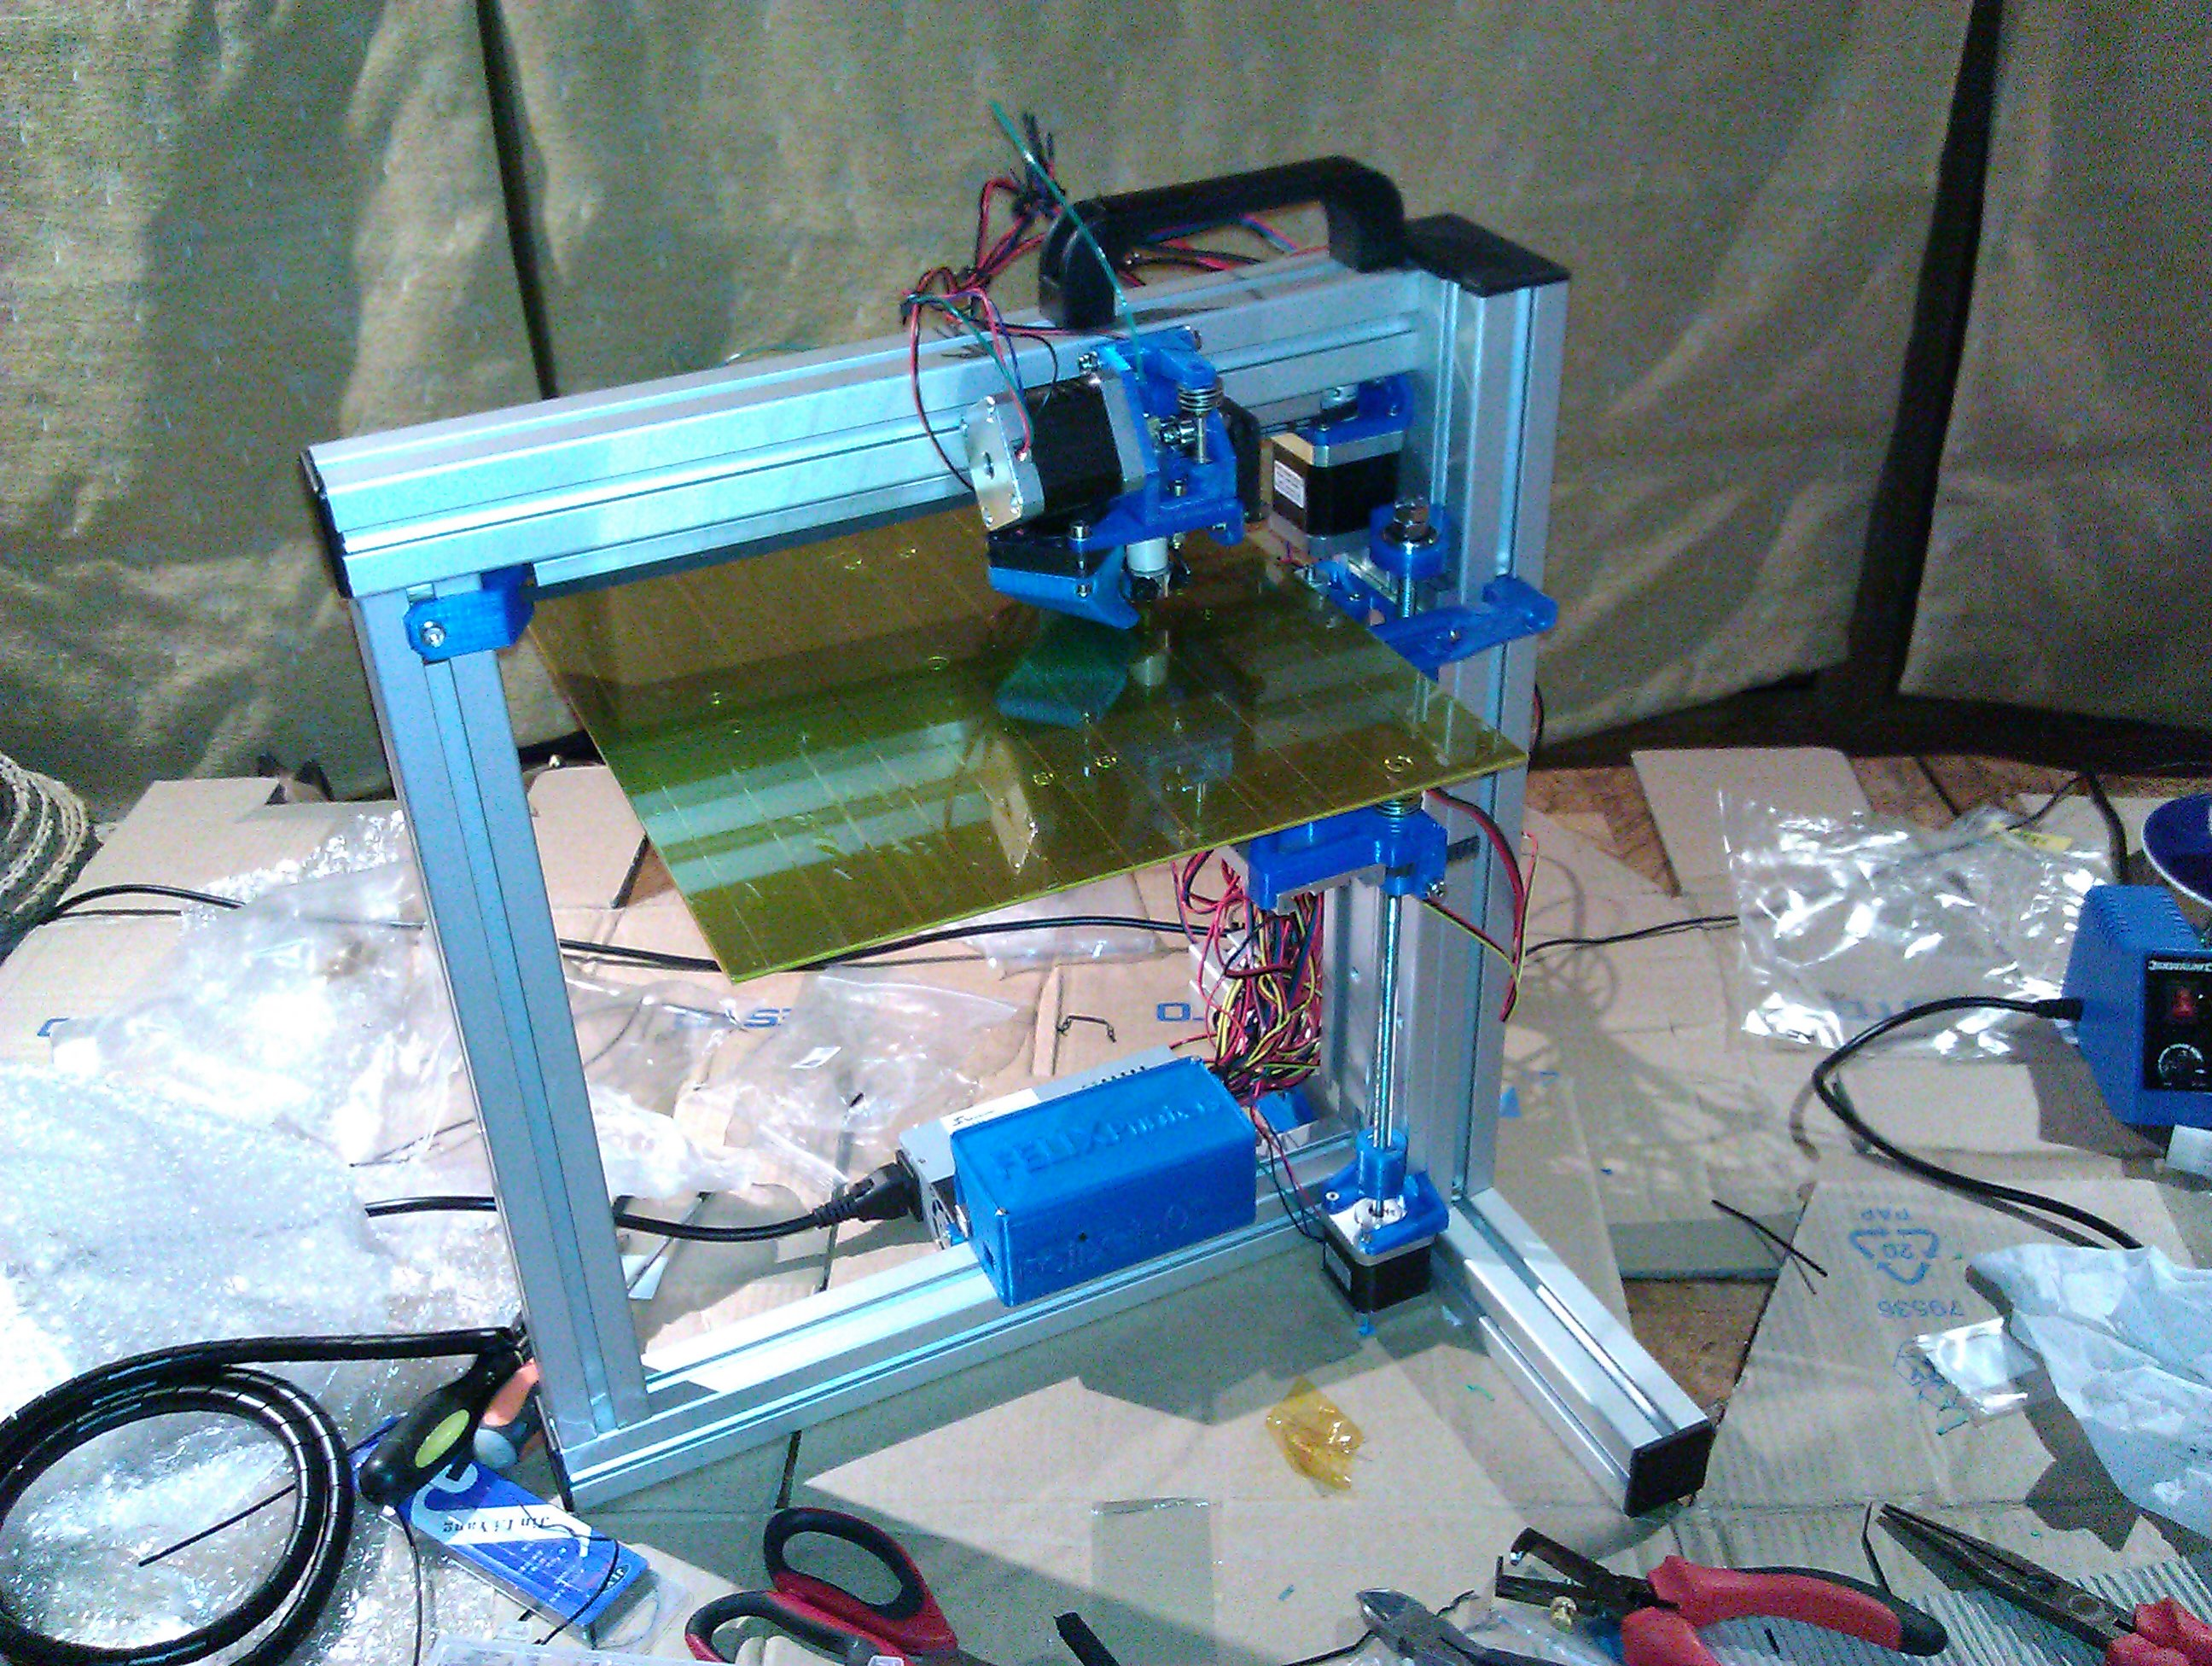
\includegraphics[width=5.0in] {figures/printer.jpg}
        \caption{3D Printer}
        \label{3D Printer}
\end{figure}



\subsection{Initial Learning}
After choosing to use the arduino due to it having such a vast amount of support and examples I bought one and began to learn how to use it, using the arduino website itself as a guide (arduino.cc).  On here there are many tutorials with circuit diagrams and example code on how to get the basics working, which I found very helpful.
\\The first things to learn were how to interact with the development board from my computer, then move onto getting it to output something.  Making lights blink was easy, and communicating over a serial connection was also relatively easy.  It got a bit harder when trying to recieve useful input from a sensor.
\\The first input I recieved was from an Infra Red sensor, using this to determine how far an object was from the sensor itself.
\\Something I discovered very quickly was that even if the sensor was not moved and the object it is pointing at is not moved the valus recieved from the sensor vary.  This 'noise' could cause a problem.  The obvious solution was to take a range of samples and average them to get a less eratic reading.
\\To further add to that I may add a threshold and if the value from each reading it too different from the current average of a range of the most recent readings, then discard that value as to not push the average.

Next I moved onto motors.  I had a 9 volt DC motor in the kit that came with my Arduino starter pack.  Getting the motor to turn was very easy, just apply current to one side and have the other linked to ground.  Simple.
\\Getting the motor to turn both forwards and backwards seemed liek it would be harder.  But due to this motor runnign well off of 5 volts this was not an issue as an Arduino can output around 5 volts on its output pins and also link these pins to ground as well.  As such I can just switch which pin is ground and which is supplying voltage to change the direction of the motor.  Of course this will not be so easy for larger motors as the Arduino will not be able to supply enough voltage in this manner.  I will require a motor driver.

\subsection{Prototype}
To build the prototype I bought a small plastic chassis kit which inclided the chassis, two wheels, a caster for the rear 'wheel', two motors and two sets of gears for the motors.  All I needed to add was the microcontroler itself, a motor driver and a power source to get this running.
%add picture of tria MK-I
\begin{figure}[h]
\centering
        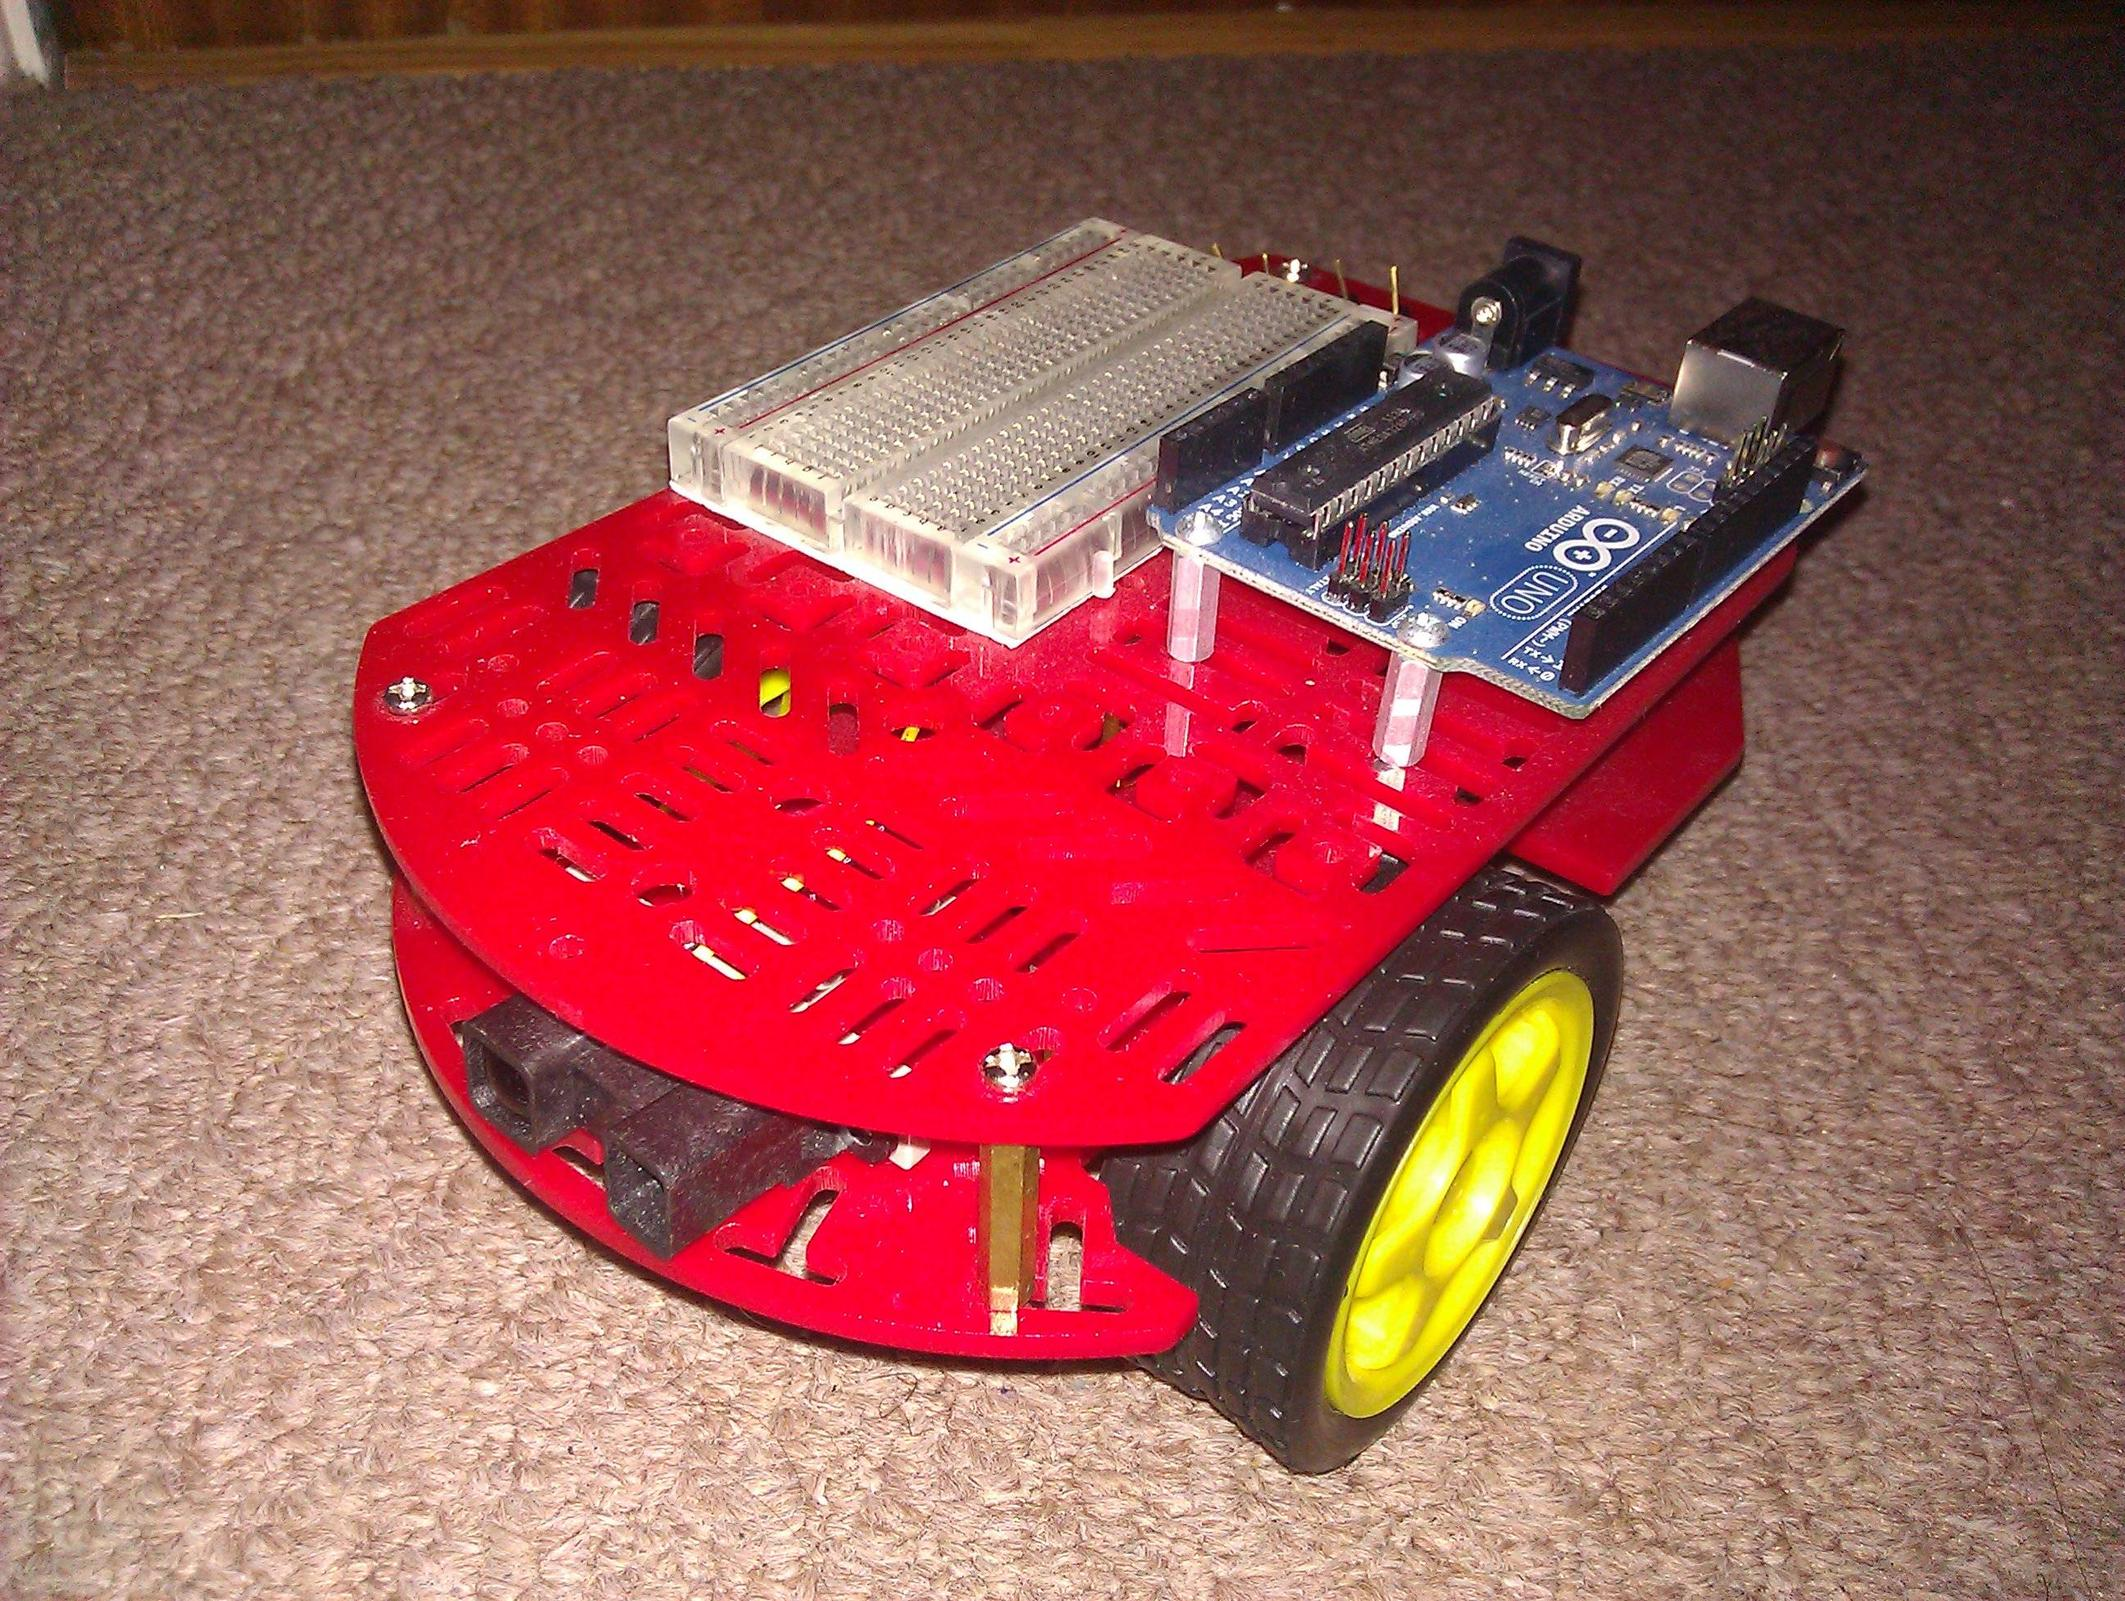
\includegraphics[width=5.0in] {figures/tria-mkI.jpg}
        \caption{Plastic prototype}
        \label{Plastic prototype}
\end{figure}
The code for the prototype was very simple and was purely for testing the concept using the device I had built.
\begin{framed}
\begin{verbatimtab}
if(sensor_range < value)
	{
		motors.turn(random);
	}else
	{
		motors.forward(1);
	}
}
\end{verbatimtab}
\end{framed}
\subsection{Current Build}
So far a basic chassis has been built out of aluminium and both the motor driver and the arduino have been mounted onto it.
\subsubsection{Base}
This consisted of cutting a sheet of aluminium to the desired shape, cutting two more pieces, bending them at a 90 degree angle and cutting a hole in them to mount the robots motors too.  These two pieces were then bolted onto the underside of the larger piece.  A further piece was bolted onto the base plate extruding out of the back to support a rear wheel.
\begin{figure}[h]
\centering
        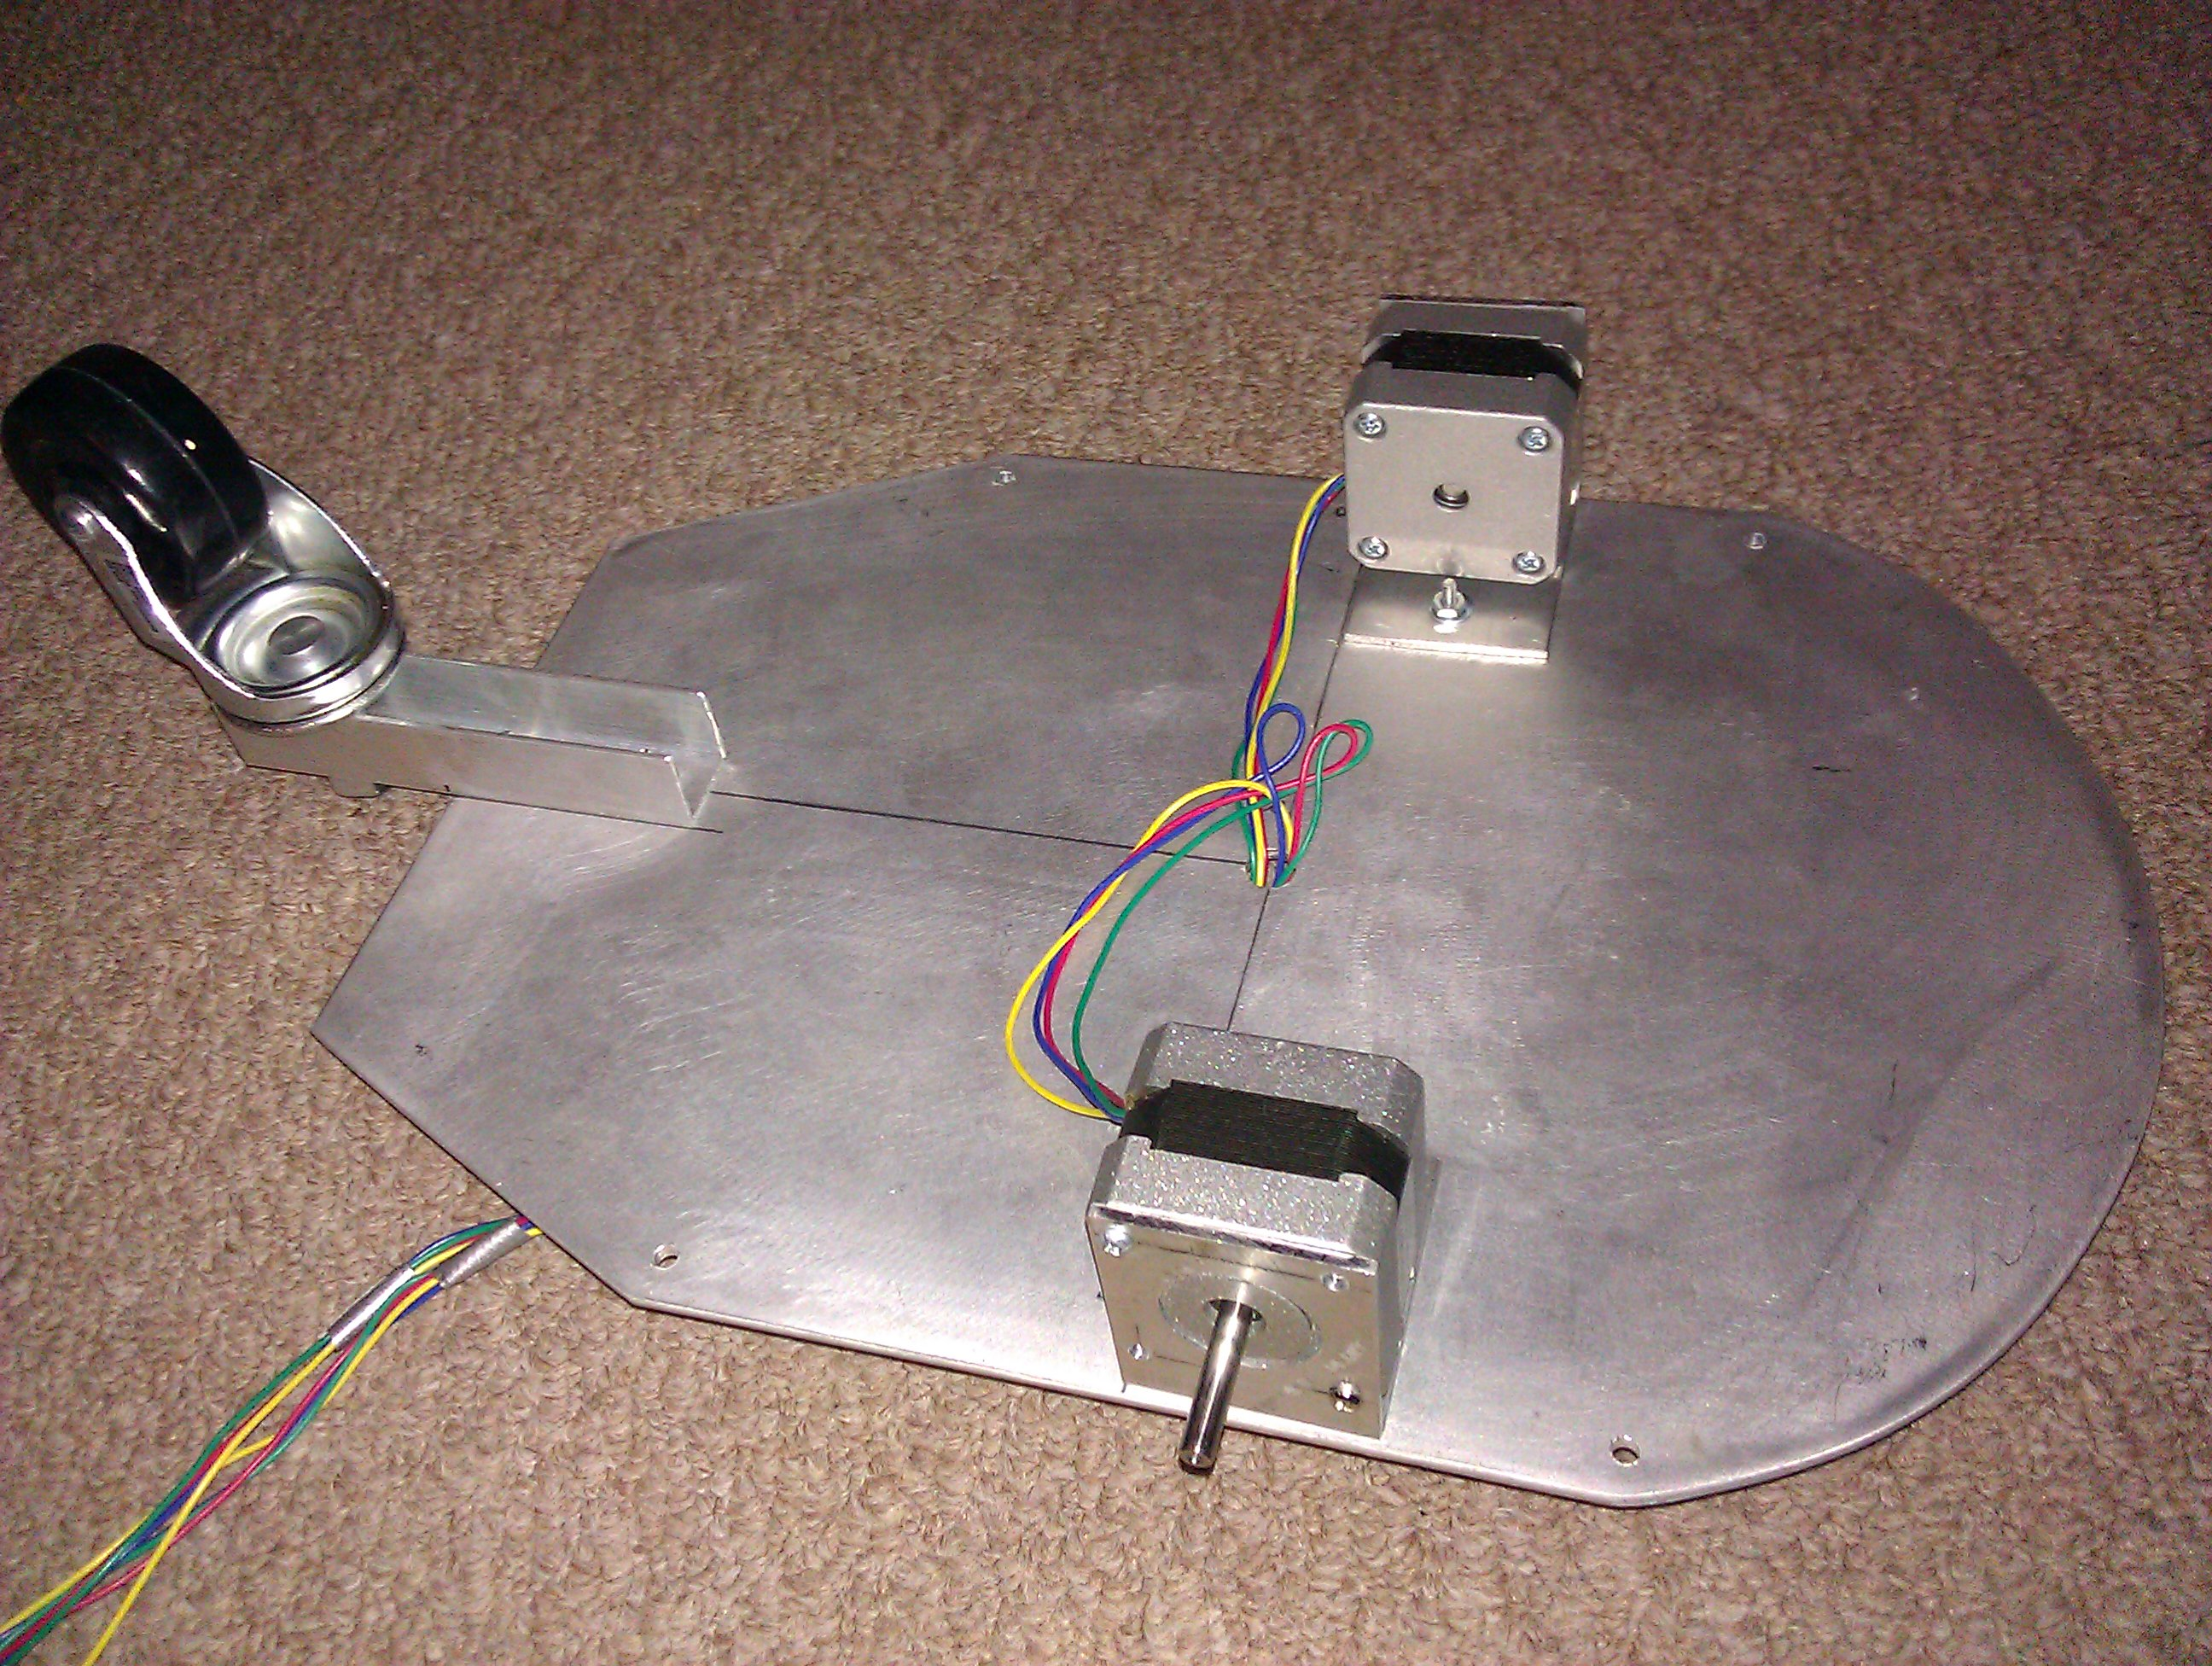
\includegraphics[width=5.0in] {figures/aluminium-chassis.jpg}
        \caption{Aluminium chassis}
        \label{Aluminium chassis}
\end{figure}

\subsubsection{Components}
Using the 3d printer I made some mounting pieces to put electronic components onto the emtal chassis.  First something small and easy.  These are a sharpe infra red sensor mount and an ultrasonic sensor mount, the models for which I downloaded off of thingiverse.
%add thingiverse reference
\begin{figure}[h]
\centering
        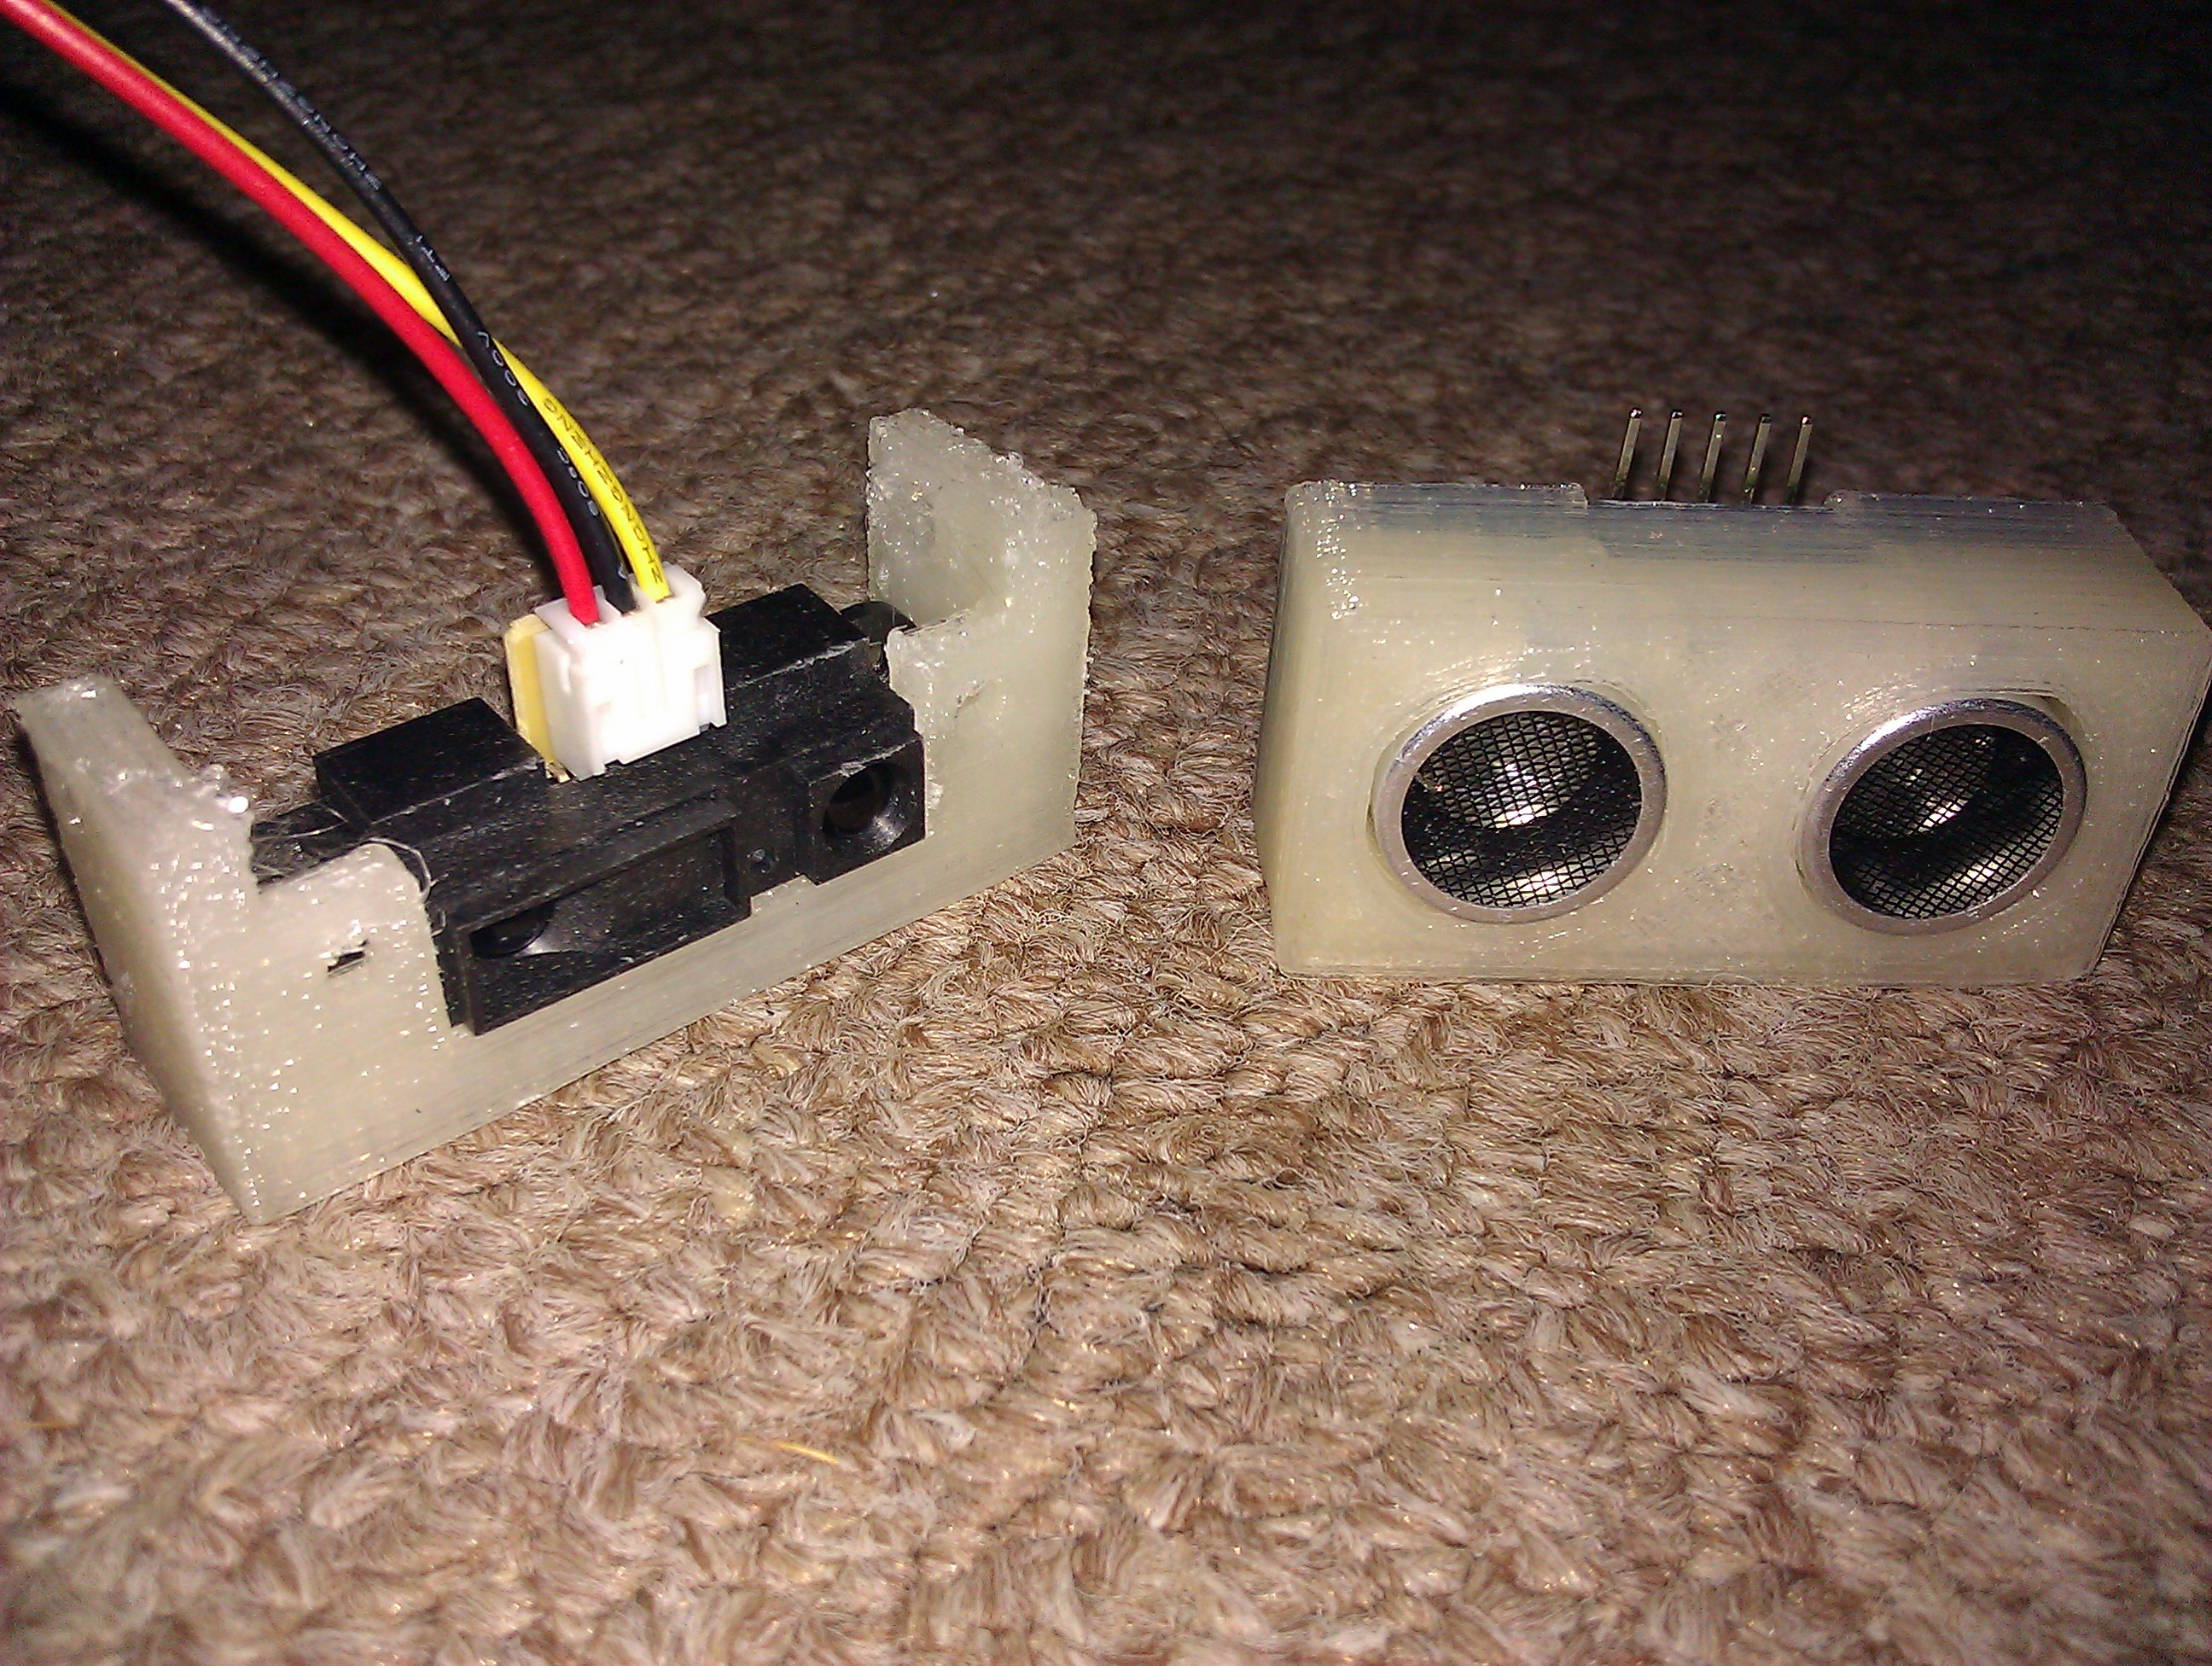
\includegraphics[width=3.0in] {figures/printed-sensor-mounts.jpg}
        \caption{Printed sensor mounts}
        \label{Printed sensor mounts}
\end{figure}
\subsubsection{Chassis}
In addition to the mounted components and the base chassis, some large wheels have been added so that it can actually drive.  These wheels are intended for off-road use and should handle and terrain the robot may end up trying to traverse.
\begin{figure}[h]
\centering
        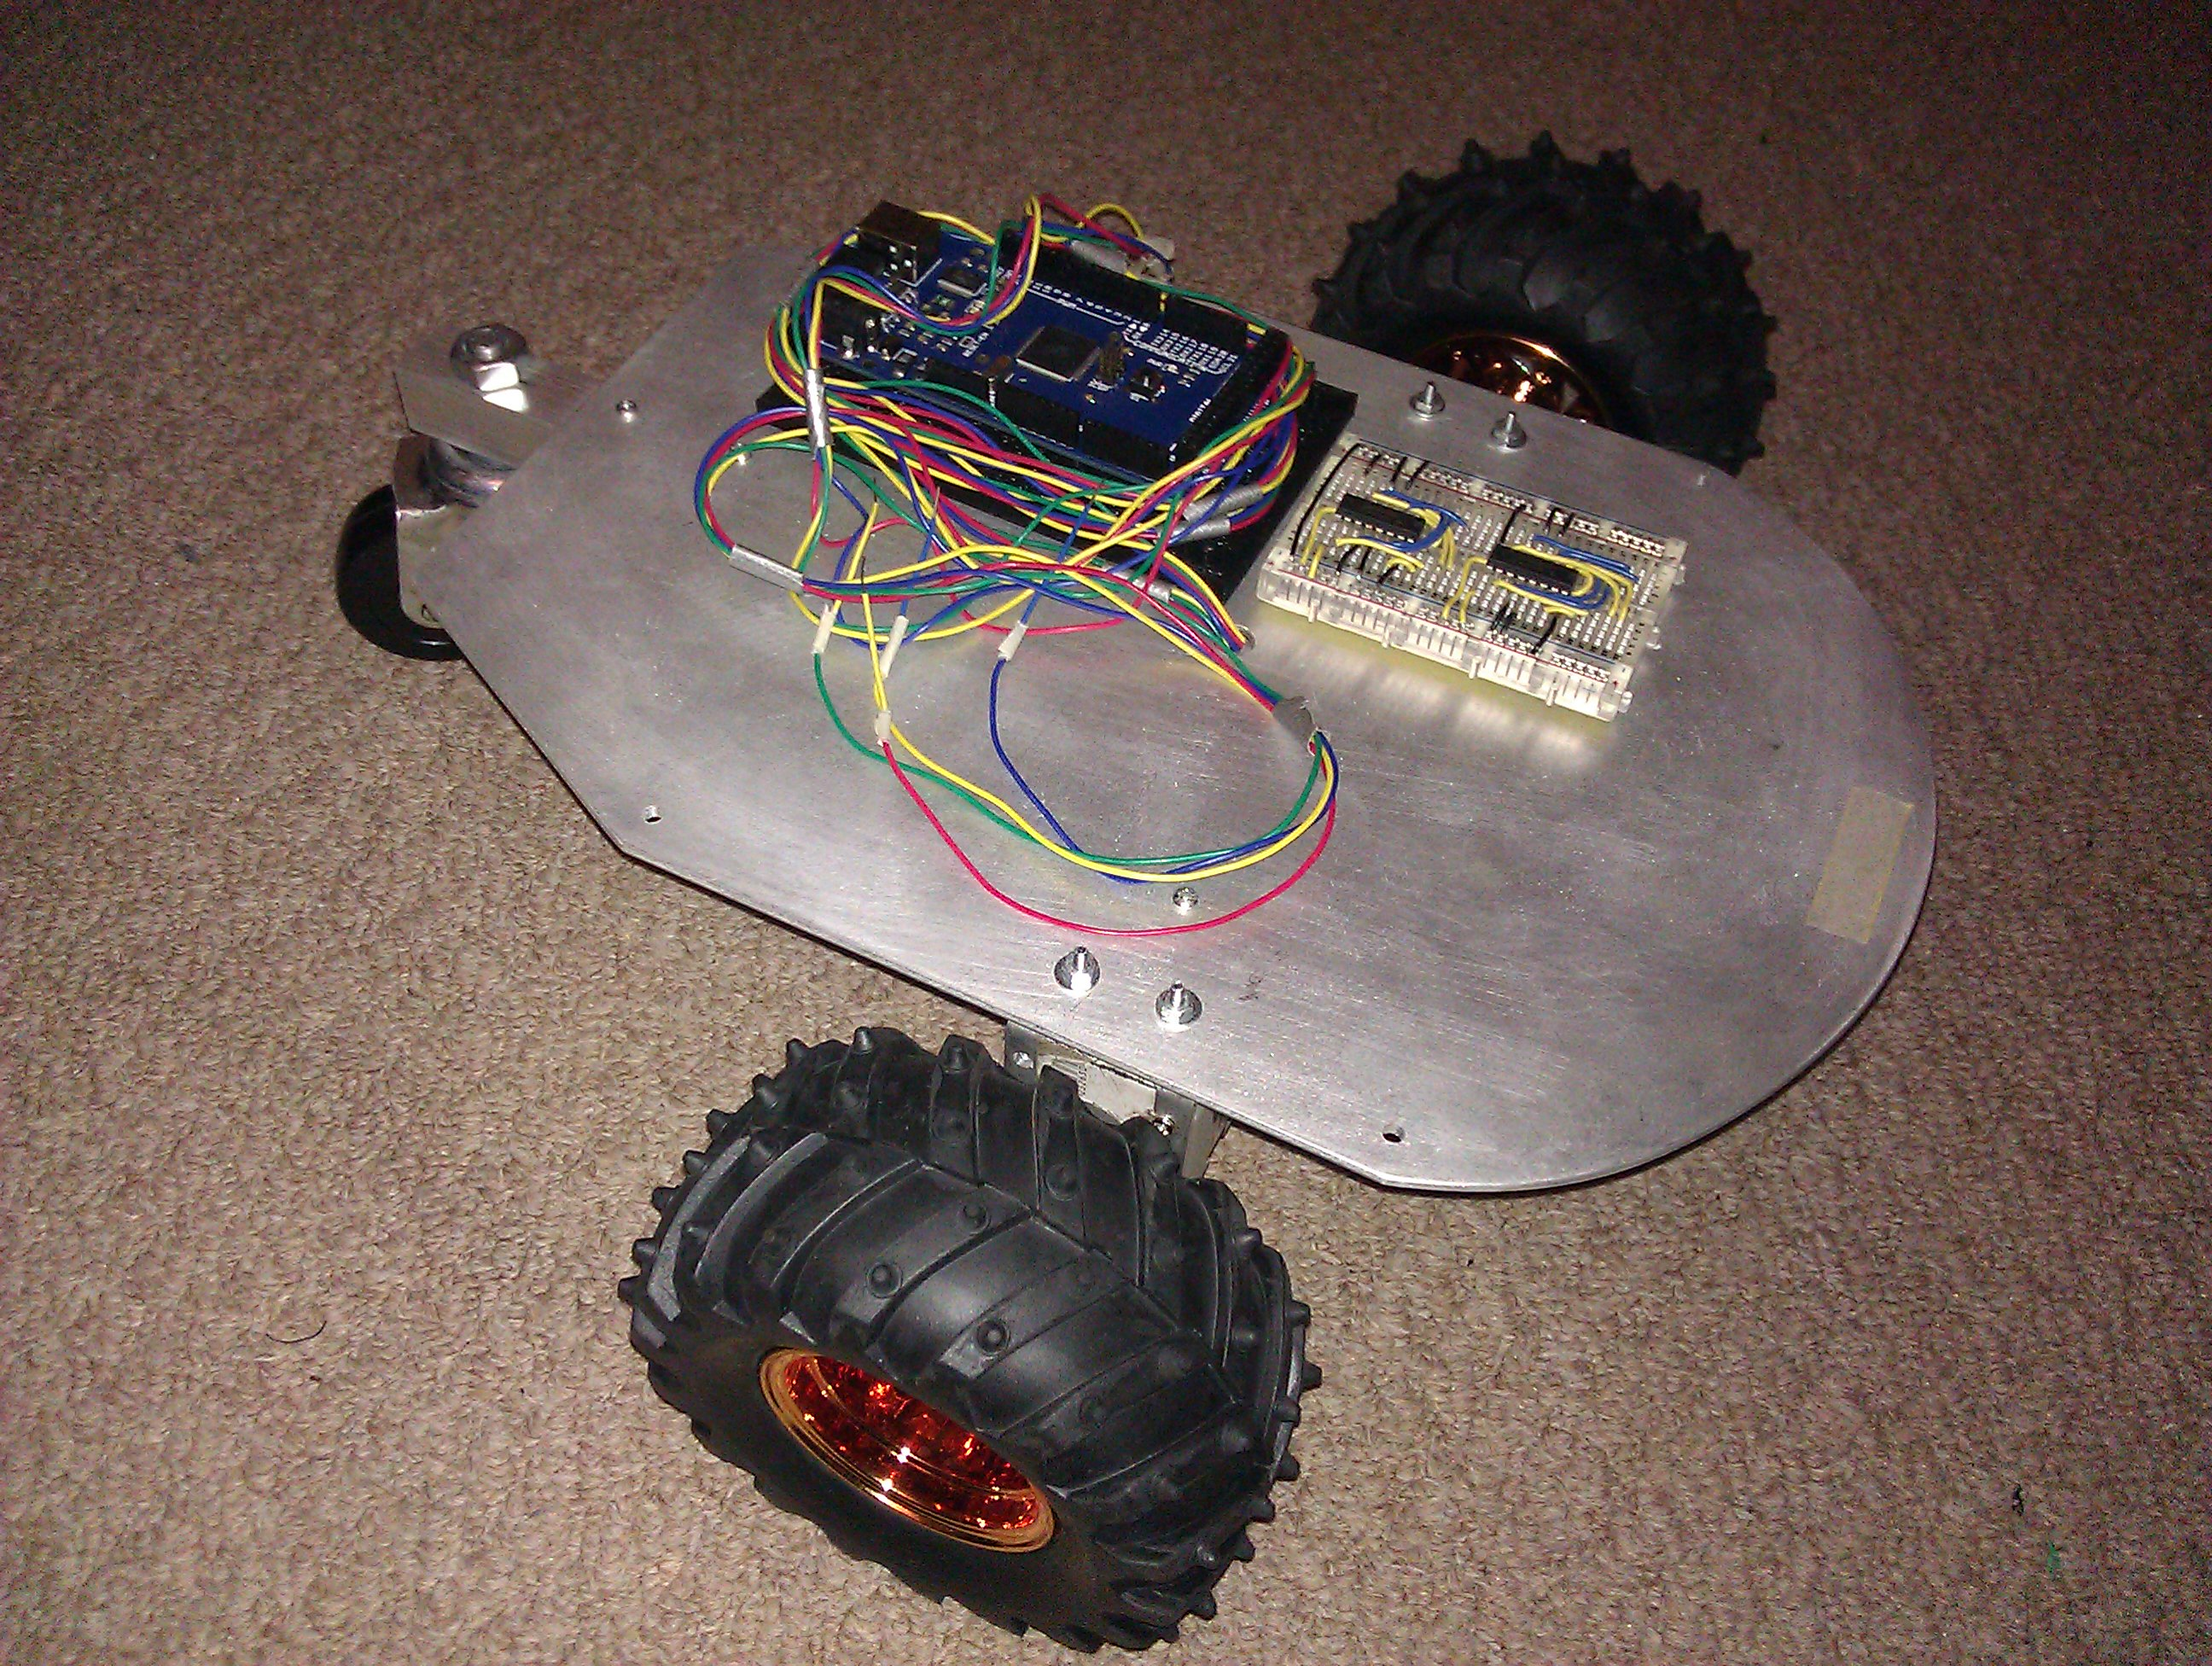
\includegraphics[width=3.0in] {figures/tria-mkII.jpg}
        \caption{Chassis with wheels}
        \label{Chassis with wheels}
\end{figure}


%==============================================================================
\section{Planning}
%==============================================================================
\subsection{Methodology}
The development methodology I have chosen is the Incremental and Iterative (IDD) approach.  This seemed apropriate due to the modular nature of this project.  To add additional functionality in each increment and repeat the whole cycle of design, build, test in every iteration.
\\Certain agile methodologies may also be apropriate but due to the prodominantly team based nature of themi rather than suited towards individuals, I chose to go with IID.
\subsection{Subsystems}
The robots functions will be divided into subsystems/modules.
\begin{itemize}
\item Controller
\\The controller unit will be a microcontroller that can recieve input from all the other devices and process what to do with the data and delegate tasks to the other systems to perform more complex tasks.
\item Motors
\\Due to the motors being steppers, they require constant control to get them to move.  Manually controllign the magnets inside the motors to get them to turn step by step or using an arduino library to it both require constant use of the microcontroller to do so.  This could be threaded or off-handed to another controller.  The off-handing approach is what I am planning.  This will take input from the control system.
\item Sensors
\\This system will constantly take sensor reading or when prompted to do so.  It will send this data to the controller to decide what to do with.
\end{itemize}
This group of basic subsystems linked together into one whole working system could be repesented by this UML (unified modeling language) diagram:
\begin{figure}[h]
\centering
	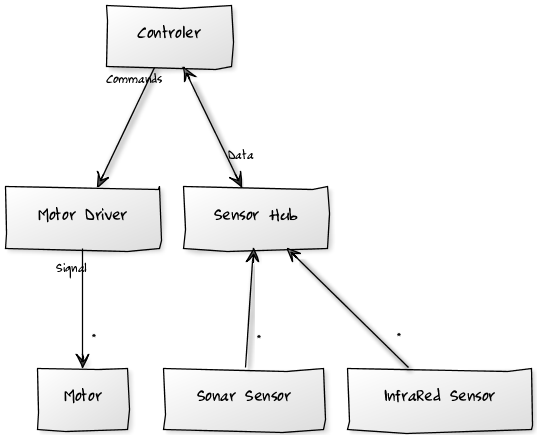
\includegraphics[width=5.0in] {figures/simple-uml.png}
	\caption{System diagram}
	\label{System diagram}
\end{figure}

\subsection{Deliverables}

\subsubsection{Progress Report}
This document which details the outline of the project, the work carried out up until the point of this document, plans for the rest of the project and background information.
\subsubsection{Mid-term Demonstration}
The mid-term demonstration should be able to demonstrate a functioning robot.  I aim to have this robot manouvering under its own power and displaying at least a basic ability to avoid large objects that may be put in its path.
\subsubsection{Final Demonstration}
For the final demonstration the aim is to build on the previous version and have the robot traversing a more complex environment on its own power and be able to send this information to a remote destination to live feedback, possibly even display some form of graphical representation of what the robot can 'see'.
\subsection{Project timeline}
The following gant chart describes the rough timeline of the project.  This includes exams, holidays and a conference.  I hope to have given plenty of time for each task as to give way for unforeseen delays and possible job interviews.
\begin{figure}[h]
\centering
        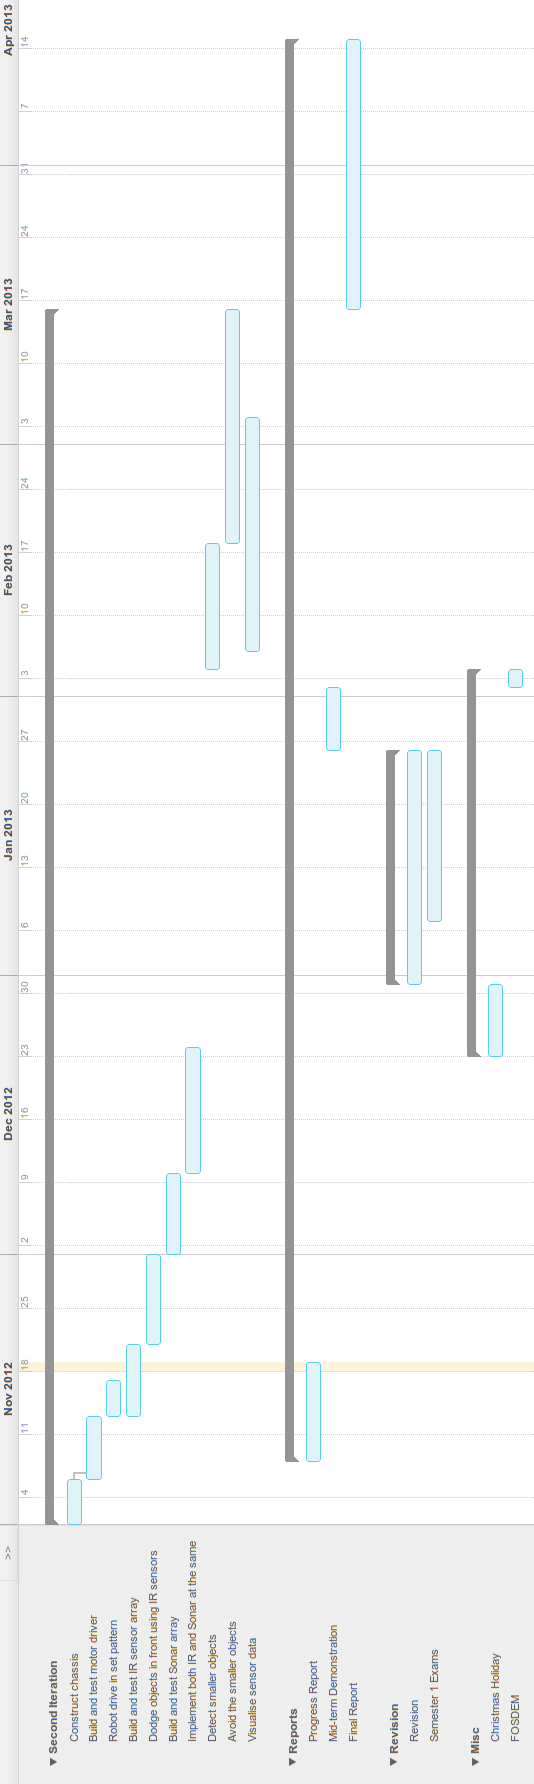
\includegraphics[width=2.1in] {figures/gant-v.png}
        \caption{Project Gant chart}
        \label{Project Gant chart}
\end{figure}
\clearpage

\nocite{*} % include everything from the bibliography, irrespective of whether it has been referenced.

% the following line is included so that the bibliography is also shown in the table of contents. There is the possibility that this is added to the previous page for the bibliography. To address this, a newline is added so that it appears on the first page for the bibliography.
\newpage
\addcontentsline{toc}{section}{Annotated Bibliography}

%
% example of including an annotated bibliography. The current style is an author date one. If you want to change, comment out the line and uncomment the subsequent line. You should also modify the packages included at the top (see the notes earlier in the file) and then trash your aux files and re-run.
%\bibliographystyle{authordate2annot}
\bibliographystyle{IEEEannot}
\renewcommand{\refname}{Annotated Bibliography}  % if you put text into the final {} on this line, you will get an extra title, e.g. References. This isn't necessary for the outline project specification.
\bibliography{mmp} % References file


\end{document}
